\begin{mdframed}[style=warning]
	\begin{ejercicio}
		\textbf{Conceptos.}
		\begin{enumerate}
			\item La figura (1) muestra la velocidad de una partícula moviendose en el eje $x$, responda
			\begin{itemize}
				\item Dirección de la velocidad inicial y final.
				\item La partícula se detiene en algún momento?
				\item La aceleración es positiva o negativa? ¿Constante o variable? 
			\end{itemize}
			\begin{figure}[H]
				\centering
				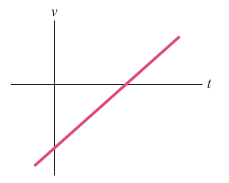
\includegraphics[scale=0.5]{./img/pregunta.png}
				\caption{}
				\label{pre}
			\end{figure}
			\item Desde o alto de un edificio se tira una pelota hacia arriba con velocidad $v_o$ y otra pelota se tira hacia abajo con velocidad $v_o$.
			\begin{itemize}
				\item ¿Qué pelota tiene mayor velocidad al alcanzar el suelo?
				\item ¿Qué pelota llega primero al suelo?
				\item ¿Qué pelota tiene mayor desplazamiento al alcanzar el suelo?
				\item ¿Qué pelota ha viajado una mayor distancia al chocar contra el suelo?
			\end{itemize}
		\end{enumerate}
	\end{ejercicio}
\end{mdframed}





\begin{mdframed}[style=warning]
	\begin{ejercicio}
		Una pequeña roca se lanza verticalmente hacia arriba con una velocidad de $18m/s$ desde la orilla del techo de un edificio de $30m$ de alto. La roca no choca contra el edificio en su trayecto hacia abajo y cae a la calle. La resistencia del aire se puede despreciar. ¿Cuál es la velocidad de la roca justo antes de caer al suelo en la calle? ¿Cuánto tiempo pasa la roca en el aire?
	\end{ejercicio}
\end{mdframed}





\begin{mdframed}[style=warning]
	\begin{ejercicio}
		Se suelta una pelota desde el techo de un edificio y pasa por una ventana, le toma $0.125s$ caer de la parte de arriba hasta la de abajo de la ventana que mide $1.2m$. Luego cae a la acera y rebota y vuelve a pasar la ventana en $0.125$. Asuma que el movimiento hacia arriba es un reverso exacto de la caída. El tiempo que la bola pasa debajo de la ventana es de $2s$. ¿Qué tan alta es el edificio?
	\end{ejercicio}
\end{mdframed}





\begin{mdframed}[style=warning]
	\begin{ejercicio}
		Dos diamantes comienzan a moverse en caída libre desde el reposo desde la misma altura, con $1s$ de diferencia uno del otro. ¿Cuánto tiempo después de que el primer diamante comienza a caer estarán los dos diamantes a $10m$ de distancia entre ellos?
	\end{ejercicio}
\end{mdframed}







\begin{mdframed}[style=warning]
	\begin{ejercicio}
		Spiderman se cae desde la parte más alta de un edificio. Si recorre la segunda mitad del edificio en $1s$, ¿Cuál es la altura del edificio?
	\end{ejercicio}
\end{mdframed}











































%%%